%---------------------------------------------------------------------------------------
%	META IMAGE
%----------------------------------------------------------------------------------------
\begin{figure}[!ht]
	\centering
	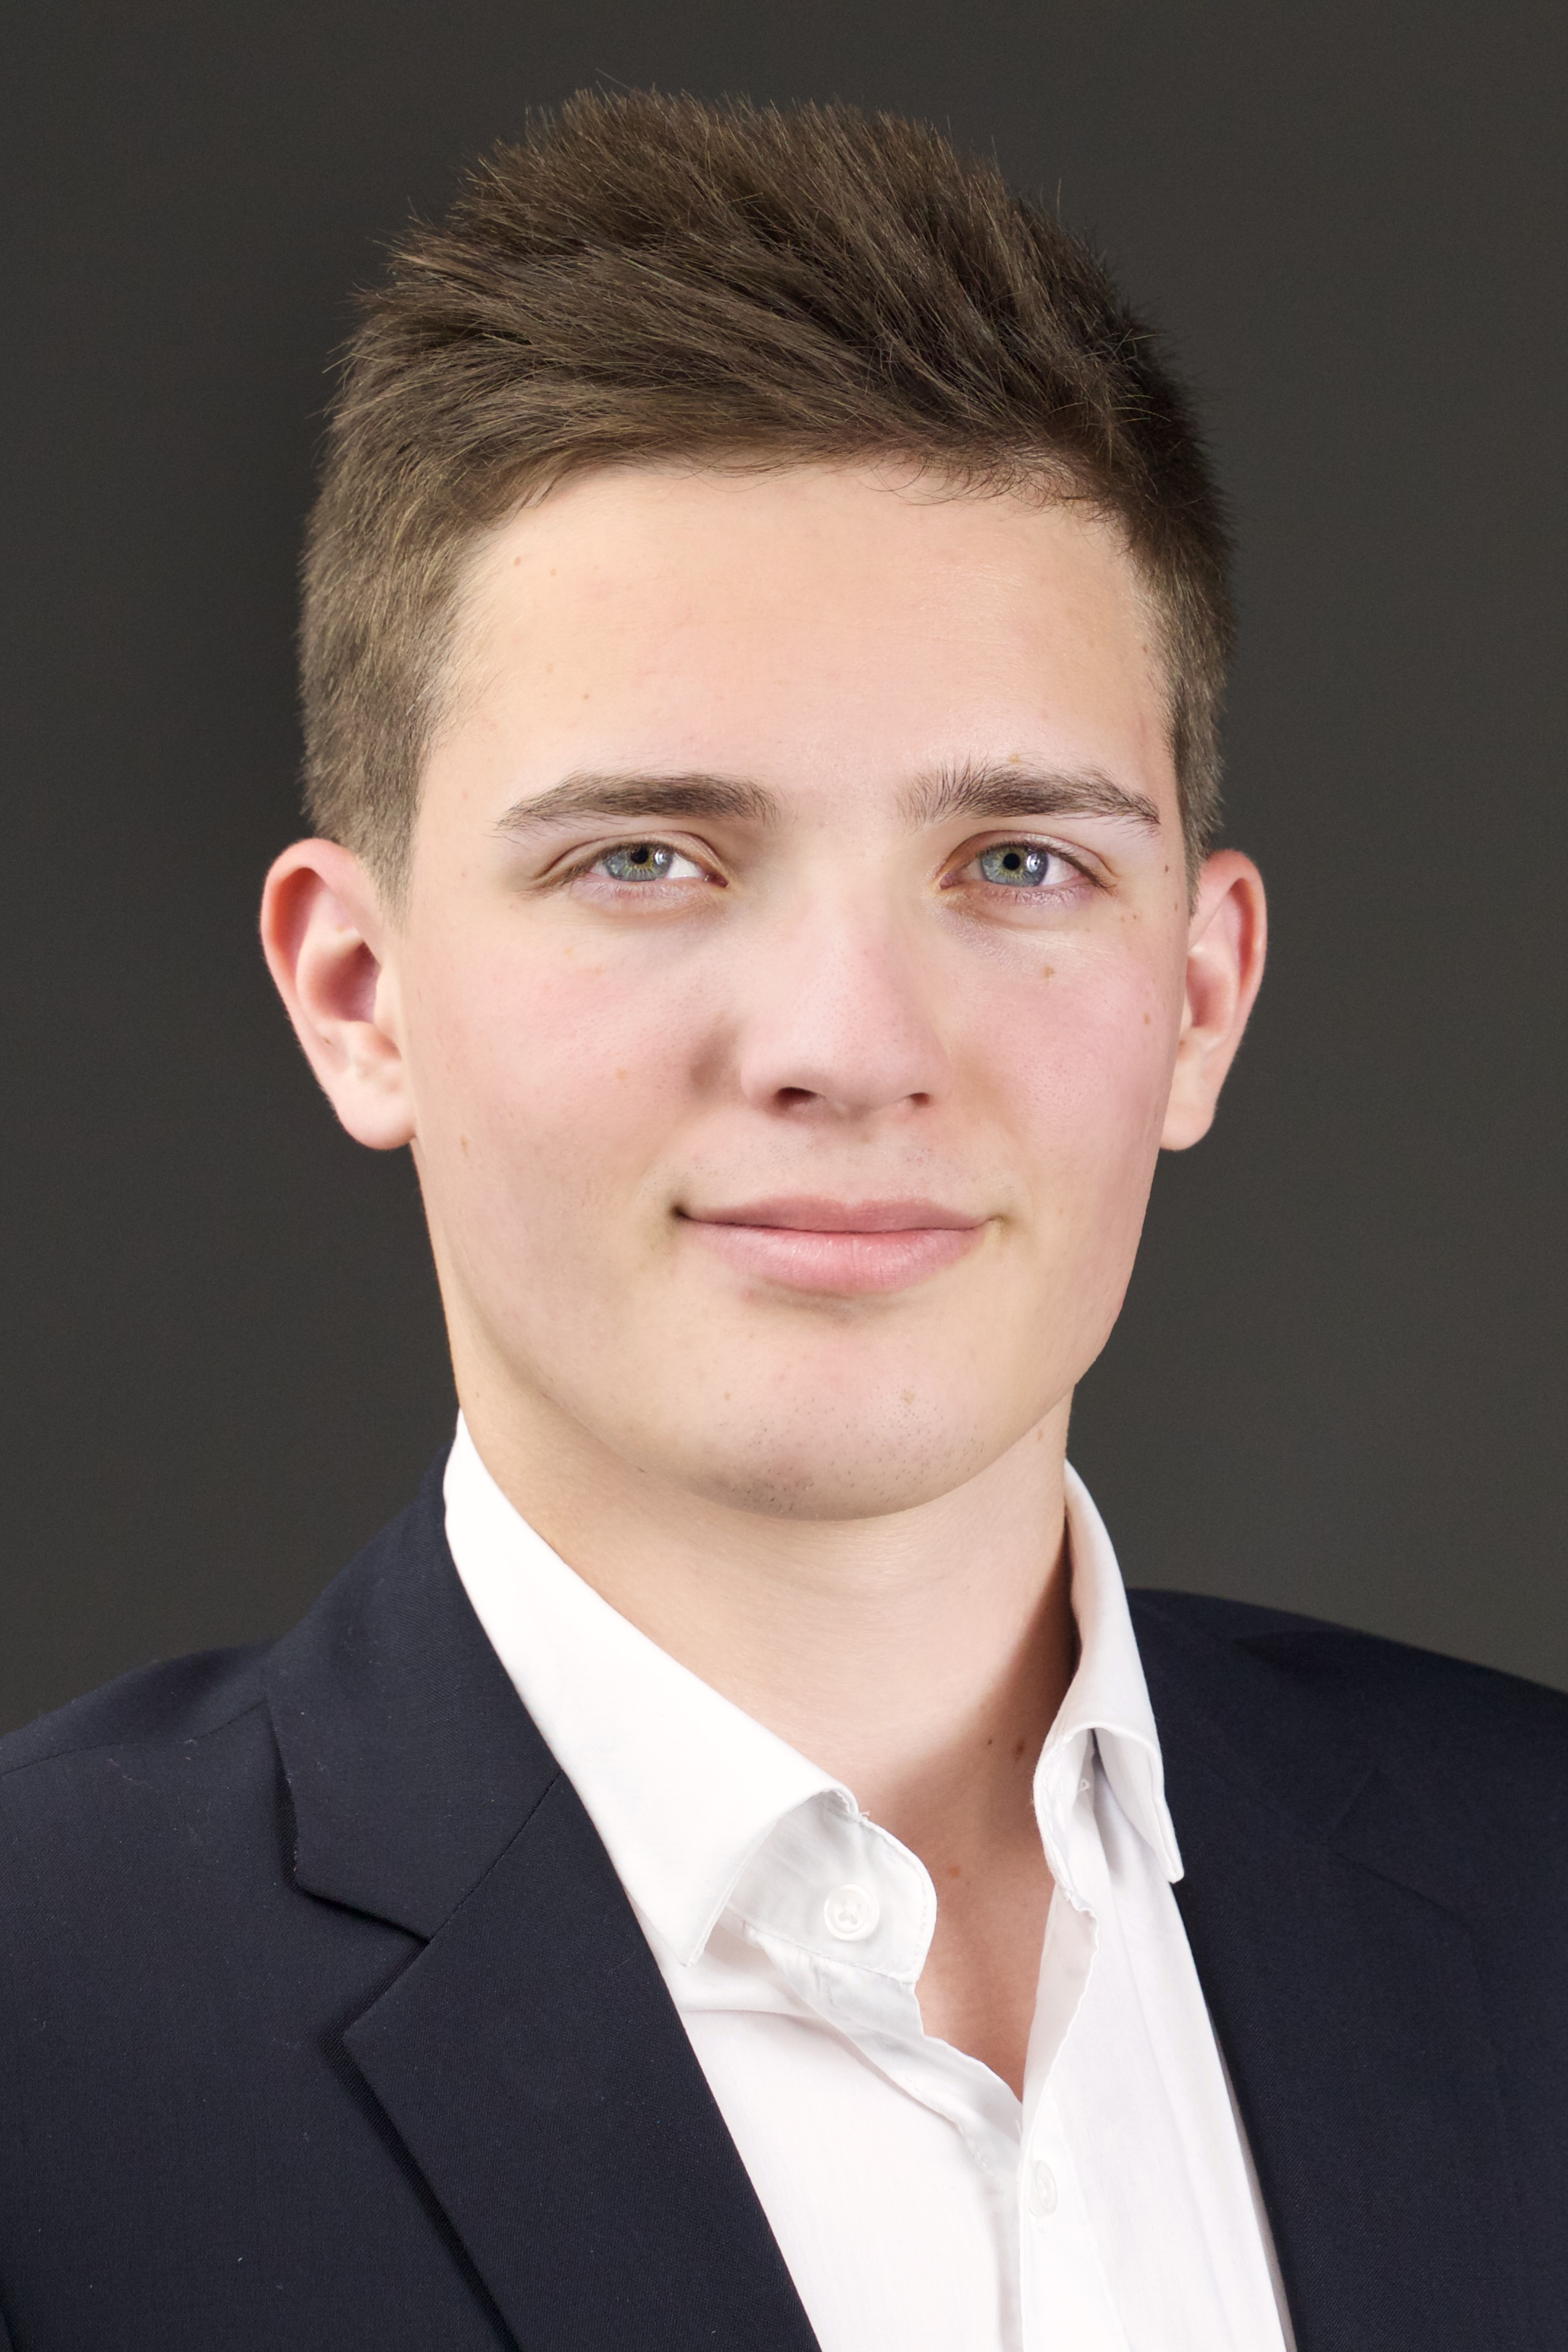
\includegraphics[width=0.95\linewidth]{../resources/visage.jpg}
\end{figure}
	%trimming relative to image size

%---------------------------------------------------------------------------------------
%	META SKILLS
%----------------------------------------------------------------------------------------
\fcolorbox{white}{white}{\begin{minipage}[c][1.5cm][c]{1\mpwidth}
		\LARGE{\textbf{\textcolor{maincol}{Dr.-Ing. Alexander\\Pfannschmidt}}} \\[2pt]
		\normalsize{ \textcolor{maincol} { Elektrische Antriebe und Maschinen} }
\end{minipage}} \\
\icontext{CaretRight}{12}{13.10.1996 in Starnberg}{black}\\[6pt]
\icontext{CaretRight}{12}{deutsch}{black}\\[6pt]
\icontext{CaretRight}{12}{ledig}{black}\\[6pt]

\cvsection{Fähigkeiten}

\cvskill{MATLAB \& Simulink} {5+ Jahre} {1} \\[-2pt]

\cvskill{Ansys Maxwell} {4+ Jahre} {0.667} \\[-2pt]

\cvskill{FEMM} {4+ Jahre} {0.667} \\[-2pt]

\cvskill{Webentwicklung} {2+ Jahre} {0.32} \\[-2pt]

\cvskill{Cloud Computing} {1+ Jahre} {0.16} \\[-2pt] \\

\cvskill{Deutsch} {L1} {1} \\[-2pt]

\cvskill{Englisch} {C1} {0.9} \\[-2pt]

\cvskill{Französisch} {B2} {0.4} \\[-2pt]

\newpage
%---------------------------------------------------------------------------------------
%	EDUCATION
%----------------------------------------------------------------------------------------
\cvsection{Bildung}
\cvmetaevent
{02/2023 -- 09/2027 | Dr.-Ing.}
{Elektrotechnik-Elektronik-Informationstechnik}
{FAU Erlangen-Nürnberg}
{Doktorarbeit: \glqq Auswirkung von Modulationsverfahren und Regelungsstrategien auf Vibrationsverhalten elektrischer Maschinen\grqq.}
\cvmetaevent
{03/2021 -- 09/2022 | M. Sc.}
{Elektromobilität und Energienetze}
{OTH Regensburg}
{Masterarbeit: \glqq Analyse unterschiedlicher Modellierungsansätze zur Bestimmung harmonischer Verluste in umrichtergespeisten permanent erregten Synchronmaschinen\grqq.}
\cvmetaevent
{10/2017 -- 03/2021 | B. Eng.}
{Regenerative Energietechnik und Energieeffizienz}
{OTH Regensburg}
{Bachelorarbeit: \glqq Entwicklung eines alternativen Q(U)-Algorithmus in PowerFactory\grqq.}
\cvmetaeventShort
{10/2014 -- 09/2016 | ---}
{Medieninformatik/Informations-\newline wissenschaft}
{Universität Regensburg}
\cvmetaeventShort
{09/2006 -- 06/2014}
{Allgemeines Abitur}
{Hans-Leinberger-Gymnasium Landshut}

\cvsection{Interessen}

\icontext{CaretRight}{12}{Rennrad}{black}\\[6pt]
\icontext{CaretRight}{12}{Fotografie}{black}\\[6pt]
\icontext{CaretRight}{12}{Bouldern}{black}\\[6pt]

\cvsection{Kontakt}

\icontext{MapMarker}{16}{Schenkstr. 75B\\91052 Erlangen}{black}\\[6pt]
\icontextHuge{MobilePhone}{16}{+49 176 31688509}{black}\\[6pt]
\iconemail{Envelope}{16}{al.pfannschmidt@gmail.com}{alexander.pfannschmidt@gmail.com}{black}\\[6pt]
\iconhref{Linkedin}{16}{linkedin.com/in/APfannschmidt}{https://www.linkedin.com/in/apfannschmidt}{black}
%\iconhref{Home}{16}{htifs.uni-regensburg.de}{http://www.ifs.uni-regensburg.de}{black}\\[6pt]
%\iconhref{Github}{16}{github.com/philipempl}{https://www.github.com/philipempl}{black}\\[6pt]
%\cvqrcode{0.3}

